\documentclass[10pt]{article}
\usepackage[a4paper,margin=2.4cm]{geometry}
\usepackage[T1]{fontenc}
\usepackage{lmodern}
\usepackage{amsmath,amssymb}
\usepackage{graphicx}
\usepackage{booktabs}
\usepackage[numbers,sort&compress]{natbib}
\usepackage{xcolor}
\usepackage[colorlinks=true,linkcolor=blue!50!black,citecolor=blue!50!black,urlcolor=blue!50!black]{hyperref}
\usepackage{caption}
\captionsetup{font=small,labelfont=bf}

\newcommand{\swtVersion}{11}
\newcommand{\swtAUC}{0.89}
\newcommand{\ifboAUC}{0.91}
\newcommand{\swtPrec}{0.66}
\newcommand{\swtRec}{0.75}
\newcommand{\ifboPrec}{0.61}
\newcommand{\ifboRec}{0.72}
\newcommand{\swtRho}{0.71}
\newcommand{\swtNear}{0.08}
\newcommand{\swtOpt}{0.62}
\newcommand{\swtSpeed}{0.49}
\newcommand{\ifboSpeed}{0.22}
\newcommand{\ifboNear}{0.01}
\newcommand{\swtMAE}{0.031}
\newcommand{\ifboMAE}{0.088}
\newcommand{\swtHB}{0.110}
\newcommand{\swtFT}{0.083}
\newcommand{\ifboHB}{0.065}
\newcommand{\ifboFT}{0.078}
\newcommand{\realHB}{0.155}
\newcommand{\realFT}{0.112}

\newcommand{\swt}{\textsf{swt}}

\title{Warped Templates: A Data-Driven Prior of Learning Curves\\for Freeze-Thaw Hyperparameter Optimization}
\author{Authors withheld (draft)}
\date{\today}

\begin{document}
\maketitle

\begin{abstract}
Freeze-thaw hyperparameter optimization (HPO) methods decide, from partial learning curves, which training runs
to continue. The strongest recent ones are trained on synthetic HPO tasks drawn from a hand-designed prior. We ask
how such a prior should look if it is built from data: we study about 570 real HPO tasks (TaskSet, JAHS-Bench-201,
QuickTune, NAS-Bench-201), each with up to 1000 configurations and full curves, and turn the findings into a
generative model. Within a task, learning curves are close to one S-shaped template in log-time that each
configuration warps: it shifts the descent in time, stretches it, and sets level and amplitude. Configurations that
never learn or that diverge occupy sharp regions along a learning-rate-like direction, and noise is heavy-tailed
and shrinks over training. The resulting prior, \swt{} (shape--warp--template), generates search spaces with a
curve for every configuration. We evaluate it on held-back task families with statistics for three separate
aspects: the shape of curves, their noise, and the landscape over configurations; and with existing HPO
algorithms. Compared with the prior used to train FT-PFN, \swt{} is closer to real data on nearly all statistics and
reproduces how much Hyperband and a freeze-thaw heuristic gain over random search far better (regret error
\swtMAE{} vs.\ \ifboMAE{}). We report the remaining gaps (landscapes too rugged, multi-fidelity gains 25--30\%
too small) and release the generator.
\end{abstract}

\section{Introduction}

Learning-curve-based HPO saves compute by training many configurations briefly and only the promising ones to
the end~\cite{swersky2014freeze,li2018hyperband,wistuba2022supervising}. Its decisions rest on a model of how a
partial curve will continue and how the curves of different configurations relate. Prior-data fitted networks
(PFNs)~\cite{muller2022transformers} learn such a model entirely from synthetic data: LC-PFN extrapolates single
curves~\cite{adriaensen2023efficient}, and FT-PFN, the surrogate of ifBO~\cite{rakotoarison2024incontext}, models a
whole task. Whatever these models believe about learning curves comes from the prior that generated their
training data. That prior is therefore a modelling decision of first importance, but it has so far been designed
by hand: in ifBO, curves are mixtures of parametric saturating families, and configurations act through a random
neural network.

This paper builds the prior from data instead. Our questions are: what do real learning curves of HPO tasks look
like, how do they vary within and between tasks, how do configurations shape them, and what does their noise look
like? Each answer becomes a part of the model, and each part is tested separately. The contributions are:
\begin{enumerate}
  \item An analysis of real HPO learning curves aimed at generative modelling (Section~\ref{sec:findings}). The
    central finding is that within a task, curves are well described by one shared template in log-time, warped per
    configuration; the apparent variety of curve shapes largely comes from the training window cutting the same
    S-shape at different places.
  \item \swt{}, a generator of synthetic HPO tasks built on this finding (Section~\ref{sec:model}).
  \item An evaluation protocol that judges a prior on three separate axes (curve shape, noise, landscape over
    configurations) plus the behaviour of existing HPO algorithms, on held-back task families
    (Section~\ref{sec:protocol}), and a development log in which every design change was measured on its own
    (Table~\ref{tab:history}).
\end{enumerate}
No HPO model is trained in this work: a prior is judged by statistics of real data and by existing HPO
algorithms. Training FT-PFN on \swt{} and testing it on the benchmarks held out in the FT-PFN paper is the next
step; those benchmarks were not touched here (Section~\ref{sec:protocol}).

\section{Related work}

\paragraph{Shapes of learning curves.} Surveys~\cite{viering2022shape,mohr2022learning} document power-law,
exponential and more complex shapes, including plateaus, peaks and non-monotone curves. Curve extrapolation
methods combine parametric families~\cite{domhan2015speeding} or learn them with Bayesian neural
networks~\cite{klein2017learning} and PFNs~\cite{adriaensen2023efficient}. We find saturating families fit HPO curves
2--8$\times$ worse than an S-shape in log-time.
\paragraph{Shape-invariant models.} Modelling a family of curves as one template with per-curve shifts and scales
is old in statistics: self-modelling nonlinear regression~\cite{lawton1972self} and SITAR for growth
curves~\cite{cole2010sitar}. We use the same idea per HPO task, in log-time.
\paragraph{Priors for freeze-thaw HPO.} Freeze-thaw BO~\cite{swersky2014freeze} assumed exponentially decaying
curves under a GP. DyHPO~\cite{wistuba2022supervising} learns a deep kernel over configurations and budgets. ifBO's
FT-PFN~\cite{rakotoarison2024incontext} is trained on a hand-designed prior; we use that prior as the baseline.
\paragraph{Benchmarks.} We use TaskSet~\cite{metz2020using}, JAHS-Bench-201~\cite{bansal2022jahs},
NAS-Bench-201~\cite{dong2020nasbench201}, QuickTune~\cite{pineda2024quicktune}, FCNet~\cite{klein2019tabular} and the
bbomix tasks of the Syne Tune blackbox repository~\cite{salinas2022synetune}. LCBench~\cite{zimmer2021autopytorch},
PD1~\cite{wang2024pretrained} and TaskSet's FixedTextRNNClassification tasks are the test benchmarks of FT-PFN and are
kept out of all our work.

\section{Data and evaluation protocol}
\label{sec:protocol}

\paragraph{Tasks.} A task is a search space, a set of configurations (up to 1000) and, for each, a learning curve
of a validation loss or error (lower is better) over $T$ steps ($T$ = 50--300). Tasks are split by family, so
that whole families are held back:
the \emph{fit} split (570 tasks used to build the model: 400 TaskSet tasks from most families, 81 JAHS-Bench-201,
86 QuickTune, 3 NAS-Bench-201) and the \emph{select} split (189 tasks used only for comparison: 150 TaskSet tasks
from the families char, conv, rnn, Associative and Copy, 4 FCNet and 35 bbomix). All model parts are fitted on fit
tasks; all numbers in this paper are measured on select tasks. A loader-level guard refuses the held-out test
benchmarks.

\paragraph{Normalisation.} Each task's curves are mapped to $z = (y - y_\text{best}) / (y_\text{ref} -
y_\text{best})$, where $y_\text{best}$ is the lowest value of any curve and $y_\text{ref}$ the 90th percentile of the
first values, so 0 is the task's best and 1 a typical starting loss; divergent values are capped at 2. A curve is
\emph{dead} if its smoothed version never falls below 0.9, \emph{diverged} if it reaches the cap or becomes
undefined, and \emph{live} otherwise.

\paragraph{Three axes and their statistics.} A prior can be right about curves and wrong about landscapes or vice
versa, so we score each aspect separately. Gaps are 1-D Wasserstein distances between the real and generated
distributions of a statistic, divided by the real standard deviation (0 = identical).
\begin{itemize}
  \item \textbf{Curve shape (B).} On curves resampled to 40 points in log-time: the log-times at which a live
    curve has made 10, 50 and 90\% of its progress; progress in the last 20\% of the budget; share of rising
    steps of the smoothed curve; largest rise after the running minimum; final value. Also a classifier two-sample
    test~\cite{lopezpaz2017revisiting} (cross-validated AUC of boosted trees telling real from generated curves; 0.5 =
    indistinguishable) and $k$-NN precision and recall~\cite{kynkaanniemi2019improved} in an 8-dimensional PCA
    embedding (precision: share of generated curves inside the real manifold; recall: the reverse).
  \item \textbf{Noise (C).} On residuals from a smoothed curve: excess kurtosis, the rate of spikes (beyond 5
    robust standard deviations), and the ratio of residual spread in the last third to the first third (gap on its
    logarithm).
  \item \textbf{Landscape (A).} Per task: \emph{predictability} $\rho_{200}$, the rank correlation between final
    values and the predictions of boosted trees trained on 200 configurations; \emph{near-best share}, the share of
    configurations within 0.05 of the best; the \emph{local-optima ratio}, local optima on a 10-nearest-neighbour
    graph relative to a random permutation of the same values (1 = as rugged as noise); \emph{speed from config},
    the cross-validated $R^2$ of predicting a live curve's time to 50\% progress from its configuration.
  \item \textbf{HPO behaviour (E).} Random search, Hyperband~\cite{li2018hyperband} ($\eta=3$) and a freeze-thaw
    heuristic run on each task with budgets of 1--20 full trainings. Regret is the rank of the incumbent's final
    value among all configurations (0 = best). We report the mean absolute difference of mean regrets from the
    real ones over algorithms and budgets (\emph{regret MAE}) and the \emph{gain} of Hyperband and freeze-thaw over
    random search (regret difference averaged over budgets). Gains have a standard error of about 0.01, so
    differences below 0.03 between priors are not meaningful.
\end{itemize}

\section{What real learning curves look like}
\label{sec:findings}

We summarise the findings that shaped the model; each was measured on fit tasks.

\paragraph{Shape: one S-shape in log-time.} Among fitted families, saturating ones (power law, exponential, Weibull)
are 2--8$\times$ worse in residual error than a two-stage S-shape in log-time, which reaches the noise floor on most
sources. Clustering curves suggests several modes (curves that only fall late, full S-shapes, curves that have
almost converged at the first observation), but these are positions of the \emph{same} S-shape relative to the
training window.

\paragraph{Within a task: one template, warped.} A shape-invariant model
\begin{equation}
  y_i(u) = \alpha_i + a_i\, f\!\big((u - \beta_i)\, e^{\gamma_i}\big), \qquad u = \log(t/T),
  \label{eq:sitar}
\end{equation}
with one smooth template $f$ per task and four parameters per curve (level $\alpha_i$, amplitude $a_i>0$, log-time
shift $\beta_i$, stretch $\gamma_i$) explains almost as much within-task variance as seven free parameters per
curve. Most shape variation lies between the configurations of a task (57--80\%); tasks within a source account for
10--17\%.

\paragraph{Configurations shape curves, not only final values.} The learning rate acts as a partial time warp plus
a level change: a higher learning rate moves a curve ahead in log-time. The configuration predicts a curve's speed
far beyond what its final value says (JAHS-Bench-201: $R^2$ 0.74 from the configuration vs.\ 0.11 from the final
value). A prior must therefore drive curve shape from the configuration, not only the final value.

\paragraph{Bad regions are organised.} Configurations that never learn (dead) and that diverge form regions that
are almost perfectly predictable from the configuration (cross-validated AUC 0.99): dead at low learning rates,
diverged at high ones, with the best configurations often right at the divergence boundary. Landscapes of final
values are smoother than random but have many local optima; the near-best region covers 3--46\% of
configurations, depending on the task.

\paragraph{Noise.} Residuals are heavy-tailed everywhere (excess kurtosis 0.5--8), skewed towards spikes in the
bad direction on some sources, not correlated in time and not shared across configurations. Their size shrinks
over training (late/early ratio 0.4--0.8) and grows with the loss level. Seed-to-seed differences are small in
general but account for 24--37\% of final-value variance among the best 10\% of configurations.

\section{The \swt{} prior}
\label{sec:model}

\begin{figure}[t]
  \centering
  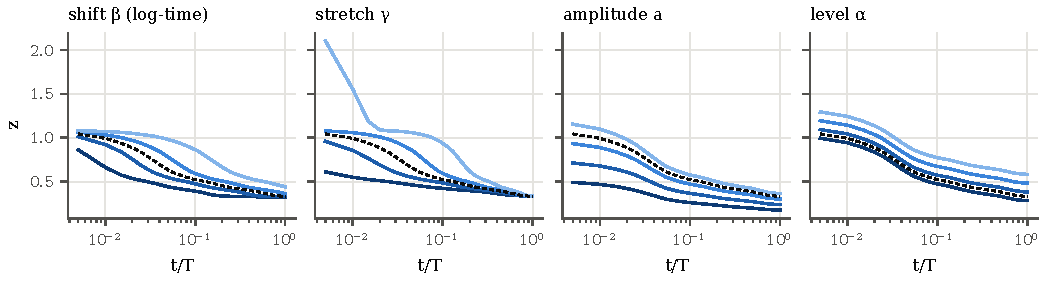
\includegraphics[width=\linewidth]{figures/model_warps.pdf}
  \caption{The four warps of Eq.~\eqref{eq:sitar} applied to a template fitted on a TaskSet task. Dashed: the
  unwarped template.}
  \label{fig:warps}
\end{figure}

\paragraph{Fitting the records.} For each fit task we fit Eq.~\eqref{eq:sitar} to all live curves of one seed. The
template $f$ is piecewise linear on 48 knots in log-time with a second-difference smoothness penalty. Fitting
alternates between an exact penalised least-squares step for $f$ and a per-curve grid search over
$(\beta_i,\gamma_i)$, with $\alpha_i$ and $a_i>0$ in closed form. The template is held flat outside the range of
template time that the real curves cover, so it is never extrapolated. Each fitted task becomes a \emph{record}:
the template, the empirical joint distribution of warp vectors, the dead and diverged shares, the dead level, the
empirical divergence times, the noise level and its profile over the budget (from robust step-to-step differences),
the tail weight of the noise (Student-$t$ degrees of freedom from the residual kurtosis), and the task's landscape
predictability measured over its live configurations.

\paragraph{Generating a task.} One draw of \swt{} proceeds as follows.
\begin{enumerate}
  \item \textbf{Task.} Pick a record (weighted by source) and set the search-space dimension $d \le 10$ to that
    of the record; configurations are uniform in $[0,1]^d$.
  \item \textbf{Landscape fields.} Draw six standardised Gaussian-process fields over the configurations with a
    random Mat\'ern-5/2 kernel (random relevances per dimension, a random mix of additive and product structure).
    Field 0 decides final values; a rough companion field (length-scales $\times 0.15$) is mixed into it with a
    weight chosen so that the expected landscape predictability matches that of the record; it gives landscapes
    local structure without white-noise ruggedness. Field 1 decides speed; it is correlated with field 0 as the
    record's real final values and speeds are.
  \item \textbf{Warps.} Each configuration's final value and log-time shift $\beta$ are the quantiles of the record's
    real distributions at its field values. Amplitude and stretch come from the record's real warp vector closest
    in (final value, speed), and the level $\alpha$ is solved so that the noise-free curve ends exactly at the target
    final value. (If that curve would dip below the record's lowest fitted curve, the real vector is used as is.)
  \item \textbf{Classes.} Dead and diverged configurations are the top shares of two scores that mix the first
    configuration dimension (a learning-rate-like axis, weight 0.7) with fields 4 and 5: dead at its low end,
    diverged at its high end. Dead curves are flat at the record's dead level, expressed in the generated task's
    own normalised units; diverged curves follow their live curve until a divergence time drawn from the record and
    then sit at the cap.
  \item \textbf{Noise.} Add Student-$t$ noise with the record's degrees of freedom, scaled by its level and
    profile over the budget.
\end{enumerate}
Curves are generated, not replayed: no real curve appears in the output, and configuration--curve pairs are new.
What is reused from real tasks are the templates and the distributions of warps, class shares and noise.
Figure~\ref{fig:anatomy} shows one generated task.

\begin{figure}[t]
  \centering
  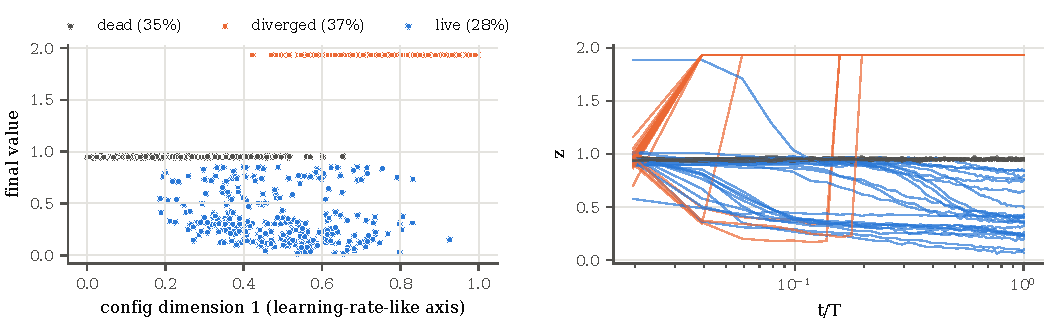
\includegraphics[width=\linewidth]{figures/anatomy.pdf}
  \caption{Anatomy of one generated task. Left: final value against the learning-rate-like configuration
  dimension; dead configurations sit at the low end, diverged at the high end, mixed with smooth fields. Right:
  a sample of its curves, coloured by class.}
  \label{fig:anatomy}
\end{figure}

\section{Results}
\label{sec:results}

\begin{figure}[t]
  \centering
  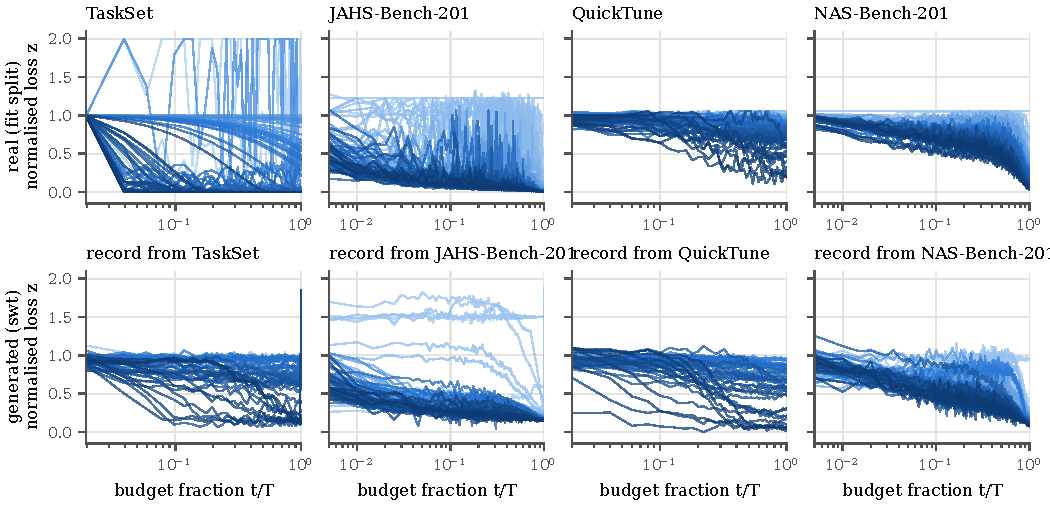
\includegraphics[width=\linewidth]{figures/examples.pdf}
  \caption{Top: real tasks from four sources (fit split, one seed, 80 random configurations). Bottom: tasks
  generated by \swt{}, each from a record of the source above it (template and parameter distributions from that
  source; configurations, landscapes and curves are new). Colour: final value (dark = good). The $x$-axis is logarithmic.}
  \label{fig:examples}
\end{figure}

\begin{table}[t]
  \centering
  \small
  \caption{Per-axis statistics on the select split (189 real tasks; equal numbers of generated tasks, one seed).
  For gaps, 0 = identical distributions. For landscape statistics, the median over tasks is shown next to the real
  median. \emph{Real fit tasks} are real tasks from the fit split, an upper reference for what any prior fitted on
  them can reach; \emph{wavetable} is a non-generative baseline that re-assigns real curves of a fit task to new
  configurations along a GP field.}
  \label{tab:axes}
  \resizebox{\linewidth}{!}{\begin{tabular}{llrrrrr}
\toprule
axis & statistic & real & ifBO prior & wavetable (hgp-v5) & swt (ours) & real fit tasks \\
\midrule
B & classifier AUC real vs.\ generated $\downarrow$ & -- & 0.91 & 0.87 & 0.89 & 0.82 \\
B & precision $\uparrow$ & -- & 0.61 & 0.70 & 0.66 & 0.80 \\
B & recall $\uparrow$ & -- & 0.72 & 0.81 & 0.75 & 0.82 \\
B & gap: time to 50\% progress $\downarrow$ & -- & 0.59 & 0.08 & 0.08 & 0.16 \\
B & gap: share of rising steps $\downarrow$ & -- & 0.36 & 0.31 & 0.05 & 0.27 \\
B & gap: final value $\downarrow$ & -- & 0.27 & 0.11 & 0.17 & 0.17 \\
\midrule
C & gap: residual kurtosis $\downarrow$ & -- & 0.61 & 0.27 & 0.24 & 0.23 \\
C & gap: spike rate $\downarrow$ & -- & 0.74 & 0.84 & 0.37 & 0.69 \\
C & gap: late/early noise ratio $\downarrow$ & -- & 0.92 & 0.28 & 0.17 & 0.14 \\
\midrule
A & landscape predictability $\rho_{200}$ & 0.77 & 0.73 & 0.78 & 0.71 & 0.78 \\
A & near-best share & 0.14 & 0.01 & 0.15 & 0.08 & 0.09 \\
A & local-optima ratio & 0.46 & 0.53 & 0.71 & 0.62 & 0.55 \\
A & speed from config ($R^2$) & 0.73 & 0.22 & 0.02 & 0.49 & 0.88 \\
\bottomrule
\end{tabular}
}
\end{table}

\paragraph{Curves.} Figure~\ref{fig:examples} compares real and generated tasks. On the curve statistics
(Table~\ref{tab:axes}), \swt{} matches when curves make their progress (gaps $\le 0.1$ for the 50 and 90\% times),
how often they rise, and their final values better than ifBO's prior. A classifier still tells single curves
apart (AUC \swtAUC{} vs.\ \ifboAUC{} for ifBO); even real fit tasks reach only 0.82 against select tasks, so part
of this is a difference between task families. Precision and recall in the PCA embedding are \swtPrec{} and
\swtRec{} (ifBO: \ifboPrec{}, \ifboRec{}); this coarse embedding separates the priors less than the per-feature
gaps do.

\paragraph{Noise.} The heavy tails (kurtosis) and spike rate of real residuals are reproduced; ifBO's Gaussian
noise has no excess kurtosis at all. The late/early noise ratio of \swt{} is somewhat too small.

\paragraph{Landscapes.} ifBO's tasks have almost no near-optimal region (median near-best share \ifboNear{} vs.\
0.14) and their curve speed barely depends on the configuration ($R^2$ \ifboSpeed{} vs.\ 0.73). \swt{} gets closer on
both (\swtNear{} and \swtSpeed{}), but its landscapes are less predictable (\swtRho{} vs.\ 0.77) and more rugged
(local-optima ratio \swtOpt{} vs.\ 0.46) than real ones.

\begin{figure}[t]
  \centering
  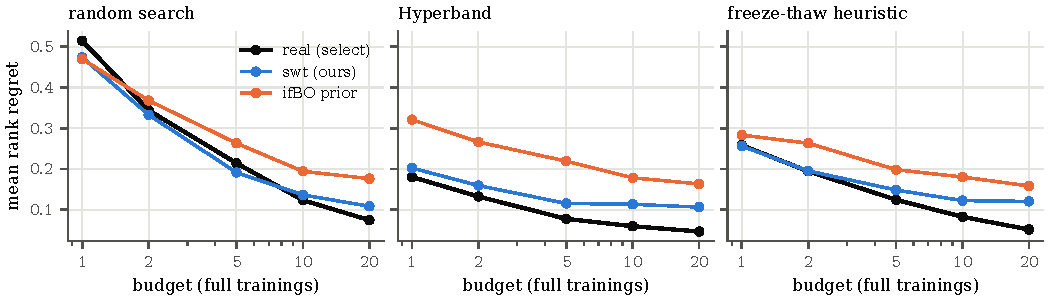
\includegraphics[width=\linewidth]{figures/hpo.pdf}
  \caption{Mean rank regret of three HPO algorithms on real select tasks, \swt{} tasks and ifBO-prior tasks.}
  \label{fig:hpo}
\end{figure}

\begin{table}[t]
  \centering
  \small
  \caption{HPO behaviour and coverage. Gains are mean regret reductions over random search ($\pm$ standard error
  over tasks). Tasks are compared through a vector of 12 standardised task descriptors (class shares, final-value
  quantiles and spread, progress times, early-rank consistency, noise level, landscape predictability).
  \emph{Coverage}: share of real select tasks with a generated task closer than the median distance between a
  real task and its nearest real neighbour. \emph{Novelty}: median distance of generated tasks to the nearest of
  600 fit tasks, divided by the same for real select tasks (0 = copies of fit tasks, 1 = as new as an unseen real
  task family). Mean over three generation seeds.}
  \label{tab:hpo}
  \begin{tabular}{lrrrrr}
\toprule
 & regret MAE $\downarrow$ & Hyperband gain & freeze-thaw gain & coverage $\uparrow$ & novelty \\
\midrule
real (select) & 0.000 & 0.155 $\pm$ 0.008 & 0.112 $\pm$ 0.007 & -- & -- \\
ifBO prior & 0.088 & 0.065 & 0.078 & 0.000 & 2.54 \\
wavetable (hgp-v5) & 0.019 & 0.130 & 0.059 & 0.150 & 0.76 \\
swt (ours) & 0.031 & 0.110 $\pm$ 0.010 & 0.083 $\pm$ 0.011 & 0.056 & 1.04 \\
real fit tasks & 0.014 & 0.140 & 0.089 & 0.178 & 0.64 \\
\bottomrule
\end{tabular}

\end{table}

\paragraph{HPO behaviour.} Figure~\ref{fig:hpo} and Table~\ref{tab:hpo} show how existing algorithms behave. On
ifBO's tasks Hyperband gains much less over random search than on real tasks (\ifboHB{} vs.\ \realHB{}), and all
algorithms keep a high regret at large budgets. On \swt{} tasks regrets follow the real ones closely (regret MAE
\swtMAE{} vs.\ \ifboMAE{}). The gains of Hyperband and freeze-thaw are still 25--30\% smaller than on real tasks
(\swtHB{} and \swtFT{} vs.\ \realHB{} and \realFT{}): early rankings are less consistent in generated tasks than in
real ones. Part of this gap cannot be closed by a prior fitted on the fit split: on TaskSet, select families have
more consistent early rankings than fit families (rank correlation of the value at 10\% of the budget with the
final value: 0.90 vs.\ 0.87).

\paragraph{Which design choices mattered.} Table~\ref{tab:history} lists the development of \swt{}, one change at a
time. Driving speed by its own field (v2) and making the unpredictable part of the landscape spatially coherent
(v3) raised speed predictability from 0.13 to 0.49; restricting the rough part to final values (v8) kept it there
after later changes. Fitting warps on all live curves rather than a subset (v5) made HPO gains closest to real but
lowered landscape predictability. Expressing the dead level in each generated task's own normalised units (v11)
fixed a defect by which a quarter of TaskSet-like tasks lost most of their dead configurations; it raised landscape
predictability to its highest value (0.71) and made dead shares follow the fit tasks.

\begin{table}[t]
  \centering
  \scriptsize
  \caption{Development of \swt{}, one change per version, measured on the select split (v6, a re-weighting with no
  measurable effect, is omitted). Precision / recall: curve axis; $\rho_{200}$, speed $R^2$, optima: landscape axis
  (medians over tasks); gains: HPO behaviour (one generation seed; standard error about 0.01).}
  \label{tab:history}
  \resizebox{\linewidth}{!}{\begin{tabular}{llrrrrrr}
\toprule
version & change & precision & recall & $\rho_{200}$ & speed $R^2$ & optima & HB / FT gain \\
\midrule
real & & & & 0.77 & 0.73 & 0.46 & 0.155 / 0.112 \\
\midrule
v1 & template + warps; vectors assigned in strata along one field & 0.61 & 0.74 & 0.70 & 0.13 & 0.72 & 0.136 / 0.106 \\
v2 & speed as its own correlated field (nearest real vector) & 0.63 & 0.76 & 0.72 & 0.37 & 0.77 & 0.133 / 0.087 \\
v3 & unpredictable landscape part spatially rough, not white & 0.66 & 0.73 & 0.72 & 0.49 & 0.66 & 0.121 / 0.070 \\
v4 & noise level from step differences, not fit residuals & 0.66 & 0.69 & 0.72 & 0.49 & 0.66 & 0.123 / 0.069 \\
v5 & warps from all live curves (no duplicated vectors) & 0.65 & 0.75 & 0.68 & 0.39 & 0.65 & 0.145 / 0.089 \\
v7 & warps constructed: exact final value and speed quantiles & 0.69 & 0.75 & 0.69 & 0.39 & 0.64 & 0.104 / 0.083 \\
v8 & rough part on the final-value field only & 0.69 & 0.74 & 0.69 & 0.50 & 0.63 & 0.107 / 0.082 \\
v9 & fallback for constructed curves below the real best & 0.69 & 0.74 & 0.69 & 0.50 & 0.62 & 0.112 / 0.086 \\
v10 & field calibrated to live configs' predictability & 0.70 & 0.75 & 0.69 & 0.49 & 0.62 & 0.109 / 0.080 \\
v11 & dead level in the generated task's own units & 0.66 & 0.75 & 0.71 & 0.49 & 0.62 & 0.110 / 0.083 \\
\bottomrule
\end{tabular}
}
\end{table}

\section{Limitations}

\begin{itemize}
  \item \textbf{Landscapes.} Generated landscapes are too rugged and not predictable enough. A diagnostic shows
    that the GP field itself is predictable (0.95); predictability is lost when dead and diverged configurations
    and noise are added, and the field's calibration does not yet account for that.
  \item \textbf{Multi-fidelity gains} are 25--30\% too small, so a method tuned on \swt{} could undervalue early
    stopping.
  \item \textbf{Templates are re-used} from fit tasks, not generated, which limits novelty in the shape of
    individual curves (task-level novelty is that of a new real task).
  \item \textbf{Not modelled yet:} minority curve patterns (two-stage plateaus, worsen-then-improve, overfitting;
    about 7\% of curves), upward-skewed spikes, several seeds per configuration, and a learned map from
    configurations to warps.
  \item \textbf{No downstream test yet.} Whether FT-PFN trained on \swt{} transfers better to the held-out benchmarks
    is the question this prior is built for; it will be evaluated once, after the prior is frozen.
\end{itemize}

\section{Using the prior}

The generator is a small Python package without deep-learning dependencies:
\begin{verbatim}
from curvefaker import faker_swt
import numpy as np
tasks = faker_swt.faker(n_tasks=100, rng=np.random.default_rng(0), version=11)
for y, X in tasks:   # y: [n, 1, T] normalised losses; X: [n, d] in [0, 1]
    ...
\end{verbatim}
The fitted records (templates, warp distributions, noise and class parameters of 570 fit tasks) ship with the
package, so no benchmark data is needed to sample.

\bibliographystyle{abbrvnat}
\bibliography{refs}

\appendix
\section{More generated tasks}
\begin{figure}[h]
  \centering
  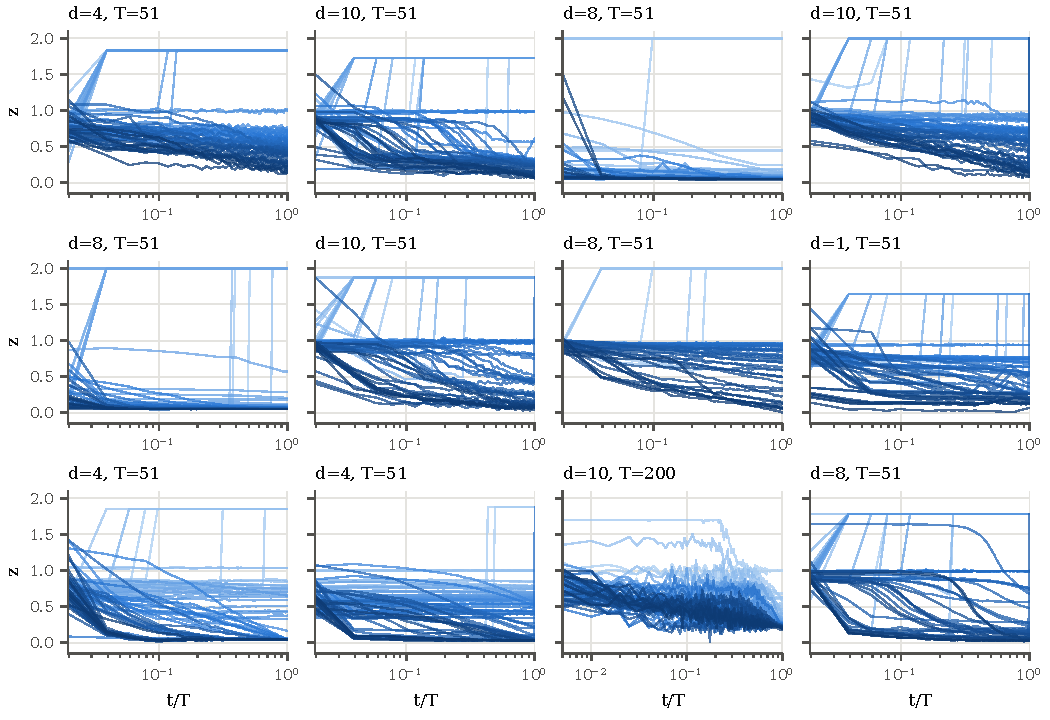
\includegraphics[width=\linewidth]{figures/gallery.pdf}
  \caption{Twelve tasks generated by \swt{} (80 random configurations each; colour: final value, dark = good).}
\end{figure}

\end{document}
